\documentclass{article}

\usepackage{amsmath}
\usepackage{amsthm}
\usepackage{graphicx}
\usepackage[backend=biber, bibencoding=utf8]{biblatex}

\addbibresource{myref.bib}

\title{Phd Computer Science Proposal}
\author{Akshay Gopalakrishnan, Clark Verbrugge \\ \\ McGill University}

\begin{document}
    \maketitle

    \section{Introduction}

         %What are memory models.
            % Give examples of SB, MP, LB, etc and relate them to existing hardwares 
        %Common problems with them addressed for each model designed 
            %-- eg: Compiler mappings correctness, Program Transformations, Robustness, Verification, etc 
        %Existing specification of models
            % Axiomatic per execution style
            % Operational 
            % Recent one -- Event structures
        %Importance of such semantic models.
            % Formal mathematical definitions of intended behaviors.
            % Verification - not our focus.
            % Help prove program transformations sound. 
            % Identify other problems with the model -- Out-of-thin-air
        %What it is lacking. 
            % Often not that intuitive
            % AXiomatic model involves several relations over events and the axioms itself are complex irreflexivity relations.
            % Operational models are abstract and could be intuitive but difficult to rely on while programming. 
            % Each model has to be proven separately for program transformations -- (WHAT DOES THIS MEAN?)
            
        This research statement is for pursuing a PhD in Computer Science under the supervision of Dr. Mark Batty. 
        The research topic is on memory consistency models. 
        A memory consistency model specifies the possible outcomes a concurrent program using shared memory can have when executed. 
        For the sake of performance, several hardware features were introduced, which sacrifice to a great extent reasoning with concurrent programming using interleaving semantics. 
        Relaxed memory models were introduced to describe such semantics.  
        These models, however have been victim to underspecified or prose specification, which has led to various problems such as compilation correctness, program transformations and a lack of understanding of the possible outcomes a program may have. 

        I propose two potential directions that can be taken to address the research problems in this domain specified by Mark Batty \cite{Batty} in his research statement.

    \section{Concurrency - Bread and Butter for Performance}

        %This should be true to your understanding and not according to someone else's 
        Almost every system we use for our day-to-day lives rely on concurrent computation. 
        Right from our mobile phones to our personal desktop which can seemingly perform multiple tasks at the same time, concurrent computations have become part of our daily life.
        The amount of performance concurrent computation has given us is something that is near impossible to part with. 
        But an important question remains, can we understand and utilize concurrency at its best for the various domain specific compuatations we intend to do? 

    \section{Memory Consistency Models - A way to tame Out-of-Order computation}


        %This section still lacks a layman's view of what is the problem of defininng memory models and its impact on other parts of programming. 

        Concurrent programs take advantage of \textit{out-of-order} execution. 
        Intuitively, this means that more than one unrelated computations can be done ``simultaneously'' without having any fixed order in which they should happen.
        This results in concurrent programs having multiple different outcomes.
        In terms of concurrenct compuations using shared memory, the possible outcomes are described by
        a \textit{memory consistency model}. 
        
        %The advent of concurrency and shared memory concurrency.
        Desipte the elaborate different ways in which we can think of writing programs that leverage the \textit{out-of-order} notion, most programmers are accustommed to reasoning about compuations sequentially. 
        Sequential Consistency(SC), which was a memory model first formulated by Lamport et al.~\cite{Lamport79}, gives programmers this exact sequential reasoning for their programs running in a multiprocessor environment.
        
        Though SC seems to be a very intuitive way to reason about programs using shared memory, it does not reflect how different processors do their computation.
        Hardwares in today's era have multiple features such as caches, read/write buffers, speculative execution, etc. which are designed to give us the performance we quite often take for granted these days.
        Usage of such features however, does not respect SC reasoning.
        For instance, consider the sample program in Fig \ref{Fig1} (in common literature known as WB or write buffering litmus test) and its possible outcomes under sequential consistency.

        %Show example here of write buffering.
        \begin{figure}
            \centering
            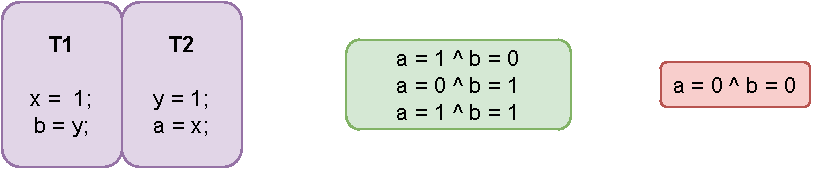
\includegraphics[scale=0.7]{WriteBuffer.pdf}
            \caption{Program with its allowed (green box) and disallowed(red box) behaviors under SC}
            \label{Fig1}
        \end{figure} 

        The disallowed outcome, however is something that can be seen for instance, in an x86 processor. 
        It is possible due to usage of write buffers that delays the visibility of writes to $x$ and $y$ to other processors / threads.
        %Mention that the disallowed outcome can be explained in terms of write buffering which is done by x86 Multiprocessors

        For high level languages, SC also implies that basic program transformations that the compiler aggressively performs may be invalidated. 
        For instance, the above disallowed outcome under SC can be justified by the compiler by just reordering independant reads and writes as shown in Fig \ref{Fig2}.

        %Show figure here with a sequential explaination of the transformed program to justify the results.
        \begin{figure}
            \centering
            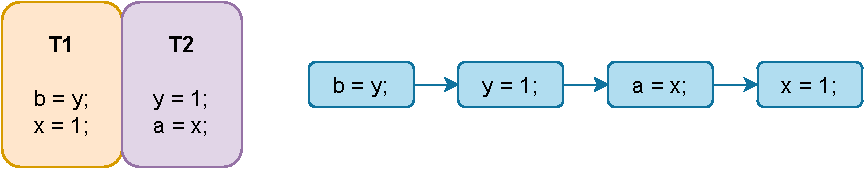
\includegraphics[scale=0.7]{ReadWriteReord.pdf}
            \caption{The above program with read-write reordered in the first thread, resulting in justifying the disallowed outcome under SC}
            \label{Fig2}
        \end{figure} 

        The above concerns called for concise formal descriptions of the behaviors shown by hardwarwe. Using such a description, we then can, giving enough freedom for compilers, give a formal description for the behaviors we would want our high level languages give the users to leverage.
        As simple as the above objective sounds, it is still quite an open ended problem.

        \section{Common Problems with Memory Consistency Models}

        Hardware vendors are notoriously known to define their system using informal prose specification.
        This has resulted in misunderstanding of what the hardware can do, which has resulted in many problems in the other layers\cite{OwensS}.
        For high level languages like Java, the initial versions of the memory model rendered even basic redundant elimination or introduction transformations invalid. This called for several revisions of the model \cite{JeremyM}. To date, the specificaiton of the Java memory model is still not completely clear and formal\cite{BenderJ}. 
        The C11/C++ memory model also faced similar problems, in addition that the model gives no guarantees for programs with Data Races, unlike that of Java \cite{BattyM}, \cite{VafeiadisV}. 
        This enables the compiler to perform any possible transformations, which  may lead to values that appear "out-of-thin-air" (although the standard out of thin air problem is described as a subset of the one we refer to. Its definition is present in the works done on C11). 
        This breaks the fundamental criteria based on which a programmer can reason with his/her programs, although its restriction would certainly disallow certain aggressive optimizations\cite{Verbrugge}. 
        Quite recently, JavaScript have also come up with their own memory consistency model, with the catch being that it is based on mixed-size memory accesses. 
        The validity of program transformations with such mixed-size accesses became a topic of investigation in my Masters program, part of which is being published \cite{Akshay}.  
        
        A lack of clear consice descriptions of the models in both hardware and software layer brought forth the daunting problem of correct compilation.
        Having incorrect compilation breaks the holy contract of the program being able to do what the user intends.
        The difficulty with the introduction of relaxed memory behaviors is that in practice, unexpected outcomes of programs happen so infrequently that it is difficult to address the correctness of compilation.   
        For instance, work done by Conrad et.al~\cite{WattC} showed that an earlier version of the JavaScript memory model, disallowed behaviors that were observable when JS programs were run in ARMv8.
        Lahav et.al~\cite{Lahav} showed a counter example to emphasize that the compilation of C11 programs to POWER were not entirely correct, even though it was formally proven in this respect.

        In the era where humans are working towards technological marvels such as self driving cars, autopilot aircrafts and spacecrafts to Mars, informal specifications itself is a problem. With the need for quick response of such systems, performance becomes an important factor and hence usage of realxed memory features becomes paramount. But their consequence due to above problems is in my view relatively more challenging as such relaxed behaviors that can occur in our programs is seen quite infrequently; one in a million or even billion runs. Hence errors can be quite devastating which might take forver to idenitfy.

    \section{Existing Forms of Relaxed Memory Specification}

        % Operational models.
        % Axiomatic Models.
        % Event structure models. 
        % Transformational - Viktor's work, show how it is different from what we want to do later.
        % Misc: pomsets with preconditions. 

    \section{Importance of the above forms of specifications}

         %Importance of such semantic models.
            % Formal mathematical definitions of intended behaviors.
            % Verification - not our focus.
            % Help prove program transformations sound. 
            % Identify other problems with the model -- Out-of-thin-air

    \section{What do the existing specifications lack}

        %What it is lacking. 
            % Often not that intuitive
            % AXiomatic model involves several relations over events and the axioms itself are complex irreflexivity relations.
            % Operational models are abstract and could be intuitive but difficult to rely on while programming. 
            % Each model has to be proven separately for program transformations -- (WHAT DOES THIS MEAN?)

    \section{Alternative Definition: Specifying Memory Models via Program Transformations}
        
        %Primary vision 
            % Towards identifying minimal set of transformations that can identify all weak memory behaviors
            % This minimal set can then be used to construct all possible memory consistency models.
            %Minimal set to perform testing of such concurrency models. 

        %Having a transformational model 
            % We start by designing memory models specified by a set of transformations allowed over a base model 
            % Doing this will give us a hierarchical structure of memory models w.r.t. program transfomraitons.
            % Intuitive to rely on by able to program justifying each outcome by some combination of program transformations.
    
    \section{Advantages}

        

        \subsection{Validating Program Transformations}

            % The set of allowed transformations can first be directly described as the set allowed for base model union the transformations we added to relax the base model.
            % We can then reason about several complex transformations by identfying the basic transformations they use from the set above.
            % Note that for this, we would also need to understand whether the set we define is basic enough to cover all complex transformations done by the compiler.

        \subsection{Correctness of Compiler Mappings}

            %If source and target model are both defined using base model M.
                % Then consider cases of the transformation sets. 
                % Transcribe from ipad notes of this.

        \subsection{Compositional Correctness}

            % Compositional reasoning can be bypassed if 
                % Both memory models under which a single program is going to be run in parts can be described using same base model M.
                % Take the intersection of their transformation sets and the intersection model is what we need to check correctness with. 

        \subsection{Robustness}

            % Analyze directly the transformation sets 
            % THe assumption here is that the source and target model can be derived from the same base model.

    \section{Challenges}

        \subsection{Part 1}

            %Identify the axiomatic elements using which we construct our base models and the transformational ones
                %Should technically account for most(ideally all) features in existing standard relaxed memory models
                %Elements should be independent of each other. (dependency will create redundancy while constructing axioms)

                %Can start off with just simple read/writes and four types of fences as defined in Doug Lea's cookbook.

            %Identify different partial/total orders required
                %ideally start off with preliminary ones.
                %Build as required.
                %May make the model more complicated aS we add on program transformations

                %Start with po, rf, mo, rb. 
                %Next one should strongly be hb.
 
        \subsection{Part 2}

            %Set of transformations
                %Mostly local 
                    %Also need to identify the granularity in each transformation (eg: Reordering how many variants? R-R, R-W, W-R, W-W or more than that)
                    %Other than reordering, elimination, introduction what other local transformations are base ones?
                    %For each local transformation, make sure that it is only w.r.t consecutive memory accesses (or redundant fences between them)
                    %This is because the non-consecutive one is just a direct inductive variant of the consecutive ones. 

                %Possible non-local 
                    %Sequentialization - merging code of two threads in either order.
                    %Parallelization - splitting a code into two threads (may not be safe in any sense)
                    %Other possibilities? Need to tread carefully as such transformations are non-trivial to understand and may affect our model construction heavily. 
                    %Having a formal definition of when we do such transformations is going to be a non-trivial endeavor. There could be many variants.
                    %Ideally, the goal is to address non-local transformations only when the local ones are all wrapped up formally and proven.


        \subsection{Part 3}

            %Defining what a transformation does.
                %based on definition, changing axiomatic definitions or modifying axioms of irreflexivity. 
                %Will definitely first change the axioms, then for convenience can add additional definitions of partial orders (like extended coherence order, writes before and what-not)
                %May need Clark's help for this phase as it can quickly go out of control.

            %Set of axioms
                %Can have various axiomatic models for same base model
                %Set of axioms should as far as possibly reflect the variants of transformations disallowed by the model itself.
                %We can start off with taking model definitions from Viktor and Ori's work.

                %In that way, allowing a transformation will ensure minimal changes in the axiomatic definition (eg: just removal of one axiom)
                %True, but it may be difficult to define the model itself as a whole, so it will be a delicate interplay between both.

        \subsection{Part 4}

            %Possibly, existing standard models may not be defined in such a way
                %Problem comes as it may be that base model M allows set T and transformed model allows T + T1, but standard model allows only T1. 
                %Then should our base model be that specific standard model? 

            %Refer to Viktor and Ori's work for more insight on this
                %Their work has proof (by counter example) that TSO cannot be defined the way we are going about, as Sequentialization is unsound under TSO but sound under SC. 
                %However, we did notice that while they discarded the possibility of defining RA being reducible (by applying sound transformations) to SC or TSO, the counter examples could be easily explained via coherence. 
                %Is it then that Coherence model is reducible to RA and models like POWER? (can perhaps ask Viktor and maybe consider doing this as a collaborative work with him)

                %Additionally, it could also be that RA can be considered as a Base model to derive Coherence by adding transformations. 
                %Is it then possible to observe any relations between multiple base models in terms of their transformation sets? 
                %This is yet to be seen and can provide really important insight, which Viktor and Ori's work has just scraped about.   


    \printbibliography

\end{document}

